\documentclass{article}
\usepackage{graphicx} % Required for inserting images

\setcounter{secnumdepth}{4}

\title{Labwork 3: Hello, CUDA!}
\author{Pham Gia Phuc}
\date{October 2024}

\begin{document}

\maketitle

\setlength\parindent{0pt}

\section{Subject}

        Make image RGB-to-gray converter using Numba CUDA \\
        • Load an image from file (matplotlib’s imread) \\
        • Flatten image into 1D array of RGB (reshape(pixelCount, 3)) \\
        • Implement grayscale using CPU (for range) \\
        • Implement grayscale using GPU \\
        • Save/show the image after each grayscale to validate the result visually \\
        • Use time.time() to measure speedup \\
        
    
\section{Implementation}
    
        This report is using CUDA kernel provided by Google Colaboratory.
        
        \begin{itemize}
            \item \textbf{Number of CUDA Devices Found:} 1
            \item \textbf{Device ID:} 0
            \item \textbf{Name:} Tesla T4
            \item \textbf{Compute Capability:} 7.5
            \item \textbf{PCI Device ID:} 4
            \item \textbf{PCI Bus ID:} 0
            \item \textbf{UUID:} GPU-af936f72-170a-716a-326e-6053e93d8f54
            \item \textbf{Watchdog:} Disabled
            \item \textbf{FP32/FP64 Performance Ratio:} 32
            \item \textbf{Multiprocessor count:} 40
            \item \textbf{Approximate core count:} 2560
            \item \textbf{Total memory size:} 14.75 GB \\
            \item \textbf{Environment:} Google Colab \\
        \end{itemize}
    

    \subsection{Result}
        The implementation process makes use of the Sample image in Figure. 1.
        \begin{figure}
            \centering
            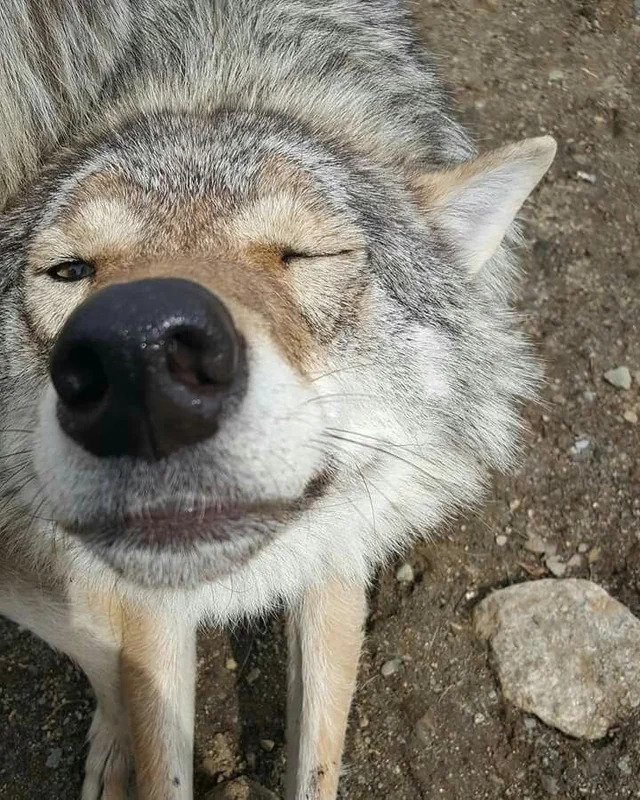
\includegraphics[width=0.5\linewidth]{wolf.jpg}
            \caption{Sample image}
            \label{fig:enter-label}
        \end{figure}

        \begin{table}[ht]
            \centering
            \begin{tabular}{@{}ll@{}}
                \textbf{CPU} & \textbf{GPU} \\
                0.043947     & 0.002064     \\
            \end{tabular}
            \caption{Processing time (seconds)}
            \label{tab:sample_table}
        \end{table}

        
\section{Conclusion}
    
    The GPU speeds up processing time by 21.29 times CPU's.

\end{document}
